\documentclass{InsightArticle}

\usepackage[dvips]{graphicx}
\usepackage{float}
\usepackage{subfigure}

\usepackage[dvips,
bookmarks,
bookmarksopen,
backref,
colorlinks,linkcolor={blue},citecolor={blue},urlcolor={blue},
]{hyperref}

\title{Smart Nearest Neighbors}

% 
% NOTE: This is the last number of the "handle" URL that 
% The Insight Journal assigns to your paper as part of the
% submission process. Please replace the number "1338" with
% the actual handle number that you get assigned.
%
\newcommand{\IJhandlerIDnumber}{3250}

% Increment the release number whenever significant changes are made.
% The author and/or editor can define 'significant' however they like.
\release{0.00}

\author{David Doria and Wanlin Zhu}
\authoraddress{Rensselaer Polytechnic Institute, Troy NY and School of Psychiatry, University of New South Wales}


\begin{document}

\IJhandlefooter{\IJhandlerIDnumber}


\ifpdf
\else
   %
   % Commands for including Graphics when using latex
   % 
   \DeclareGraphicsExtensions{.eps,.jpg,.gif,.tiff,.bmp,.png}
   \DeclareGraphicsRule{.jpg}{eps}{.jpg.bb}{`convert #1 eps:-}
   \DeclareGraphicsRule{.gif}{eps}{.gif.bb}{`convert #1 eps:-}
   \DeclareGraphicsRule{.tiff}{eps}{.tiff.bb}{`convert #1 eps:-}
   \DeclareGraphicsRule{.bmp}{eps}{.bmp.bb}{`convert #1 eps:-}
   \DeclareGraphicsRule{.png}{eps}{.png.bb}{`convert #1 eps:-}
\fi


\maketitle


\ifhtml
\chapter*{Front Matter\label{front}}
\fi

\begin{abstract}
\noindent

This document presents an implementation of two algorithms, Voronoi Neighbors and Binary Space Partition (BSP) Neighbors. These algorithms find neighbors of a point in a point set that are somehow ``better'' than a ``K nearest neighbors'' or a ``all neighbors within a radius'' query. This type of nearest neighbor query is more computationally expensive, but results in set of neighbors with more desirable properties. The BSP Neighbors search ensures that there is less local duplication, while the Voronoi Neighbors search ensures that the spatial arrangement of the neighbors is as uniform as possible.

These algorithms are explained in ``Point Primitives for Interactive Modeling and Processing of 3D Geometry''.

The code is available here:
https://github.com/daviddoria/SmartNearestNeighbors

\end{abstract}

\IJhandlenote{\IJhandlerIDnumber}

\tableofcontents
%%%%%%%%%%%%%%%%%%%%
\section{Introduction}
Defining local neighborhoods of a point is a very important step in computing local surface properties of point clouds (point sampled surfaces). Typical nearest neighbor searches (K-Nearest and PointsWithinRadius) suffer from the necessity of setting a parameter (K or the radius) to which the resulting neighborhood is very sensitive. For example, in Figure \ref{fig:KNearest} we show how with a bad choice of $K$, the resulting neighbors can be a very poor representation of the neighborhood of a point. This is not a particularly contrived case, as typically sample density varies significantly over the surface described by a point cloud.

\begin{figure}[H]
\centering
\subfigure[A point (red) and some surrounding points (blue).]
  {
  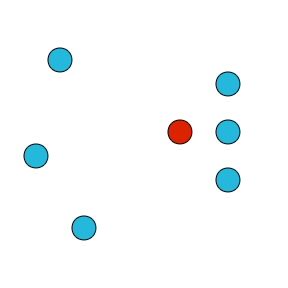
\includegraphics[width=0.25\linewidth]{images/PointAndNeighbors}
  \label{fig:KNearest:Point}
  }
\subfigure[K=3 Nearest Neighbors (green).]
  {
  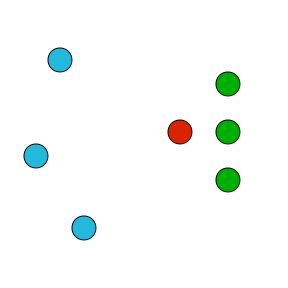
\includegraphics[width=0.25\linewidth]{images/K3Nearest}
  \label{fig:KNearest:K3Nearest}
  }
\subfigure[K=6 Nearest Neighbors (green).]
  {
  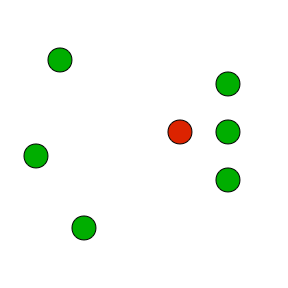
\includegraphics[width=0.25\linewidth]{images/K6Neighbors}
  \label{fig:KNearest:K6Nearest}
  }
\caption{A demonstration of the sensitivity of KNearestNeighbors to the parameter K.}
\label{fig:KNearest}
\end{figure}

In this article we present implementations of two algorithms, Voronoi Neighbors and Binary Space Partition (BSP) Neighbors. These nearest neighbor queries are more computationally expensive than the naive versions, but result in sets of neighbors with more desirable properties. These implementations are based on the algorithms described in \cite{Pauly2003}.

Figure \ref{fig:NeighborhoodComparison} compares the two algorithms we will describe to a standard K-Nearest neighbors algorithm.

\begin{figure}[H]
  \centering
  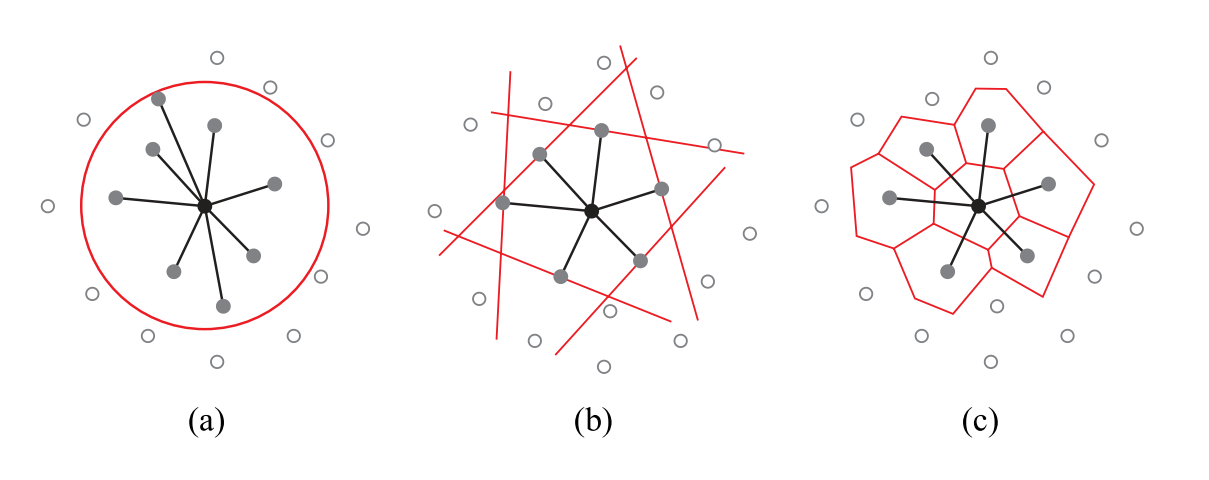
\includegraphics[width=0.7\linewidth]{images/NeighborhoodComparison}
  \caption{A comparison of (a) K-nearest neighbors, (b) BSP-neighbors, (c) Voronoi neighbors. (Taken from \cite{Pauly2003}.)}
  \label{fig:NeighborhoodComparison}
\end{figure}

%%%%%%%%%%%%%%%%%%%%
\section{Voronoi Neighbors}
The Voronoi neighbors of a point are all points whose Voronoi cell borders the Voronoi cell of the query point. This set of neighbors is spatially as uniform as possible. Figure \ref{fig:Voronoi} shows the outputs of the included Demo2D.cpp.

\begin{figure}[H]
  \centering
  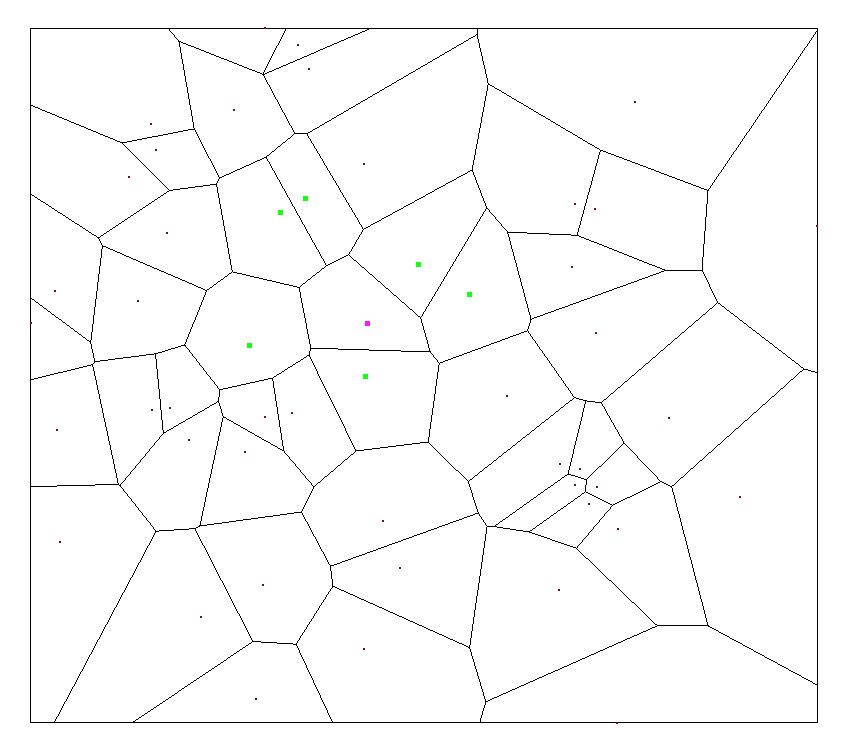
\includegraphics[width=0.7\linewidth]{images/Voronoi}
  \caption{The Voronoi diagram of a point set and the Voronoi neighbors (green) of a query point (pink).}
  \label{fig:Voronoi}
\end{figure}

All of the Voronoi computations are performed using itkVoronoiDiagram2DGenerator. We have simply provided a wrapper which takes a point set and returns the neighboring points. Note that this method currently only works with 2D point clouds, as the ITK implementation of Voronoi diagrams only works on 2D point clouds. One very strong advantage of this method of finding nearest neighbors is that there are absolutely no parameters to specify.

\subsection{Implementation Details}
Internally, itkVoronoiDiagram2DGenerator sorts the seeds (points) that are provided. This procedure changes the IDs of the points, so any information (IDs of neighboring Voronoi cells, etc) further along in the algorithm will no longer correspond to the IDs of the input points. To remedy this, we sort the input points before passing them to the Voronoi generator using the same sorting algorithm that it uses internally. We perform this sort as a parallel sort with the point IDs so that we produce a map from the new IDs to the old IDs that can be used to determine the input point corresponding to the ID of the seed at the output of the Voronoi diagram generation algorithm.

\subsection{Code Snippet}

\begin{verbatim}
// Find the Voronoi Neighbors of point 0
unsigned int queryPointId = 0;

// Create the input point set
vtkSmartPointer<vtkPoints> points2D = vtkSmartPointer<vtkPoints>::New();
... Fill points2D with points on the Z=0 (XY) plane ...

// Create an object in which to store the result
vtkSmartPointer<vtkPoints> neighbors = vtkSmartPointer<vtkPoints>::New();

// Compute the Voronoi neighbors.
VoronoiNeighbors(points2D, queryPointId, neighbors);
\end{verbatim}


%%%%%%%%%%%%%%%%%%%%
\section{BSP Neighbors}
Each nearest neighbor point defines a halfspace. The BSP neighbors are a subset of the kNearestNeighbors
which are in the intersection of all of the halfspaces induced by the kNearestNeighbor points.

To ease the explanation, we make some definitions:

\begin{itemize}
 \item $x$ a test point, any point in the space
 \item $n_i$ is the $i^{th}$ nearest neighbor point
 \item $q$ is the query point (the point for which the neighbors are being computed)
\end{itemize}

We can then define some vectors:

\begin{itemize}
 \item $v_{n_i\rightarrow q} = q - n_i$ is the vector from the $i^{th}$ nearest neighbor to the query point
 \item $v_{n_i\rightarrow x} = x - n_i$ is the vector from the $i^{th}$ nearest neighbor to a point $x$
\end{itemize}

Each kNeighbor defines a halfspace as:
\begin{equation}
v_{n_i\rightarrow q}.v_{n_i\rightarrow x} \geq 0
\end{equation}

The collection of points $x$ that satisfy this equation is exactly the positive halfspace defined by the $i^{th}$ neighbor. This equation simply says that the angle between $v_x$ and $v_{ni}$ must be less than 90 degrees. This is shown graphically in Figure \ref{fig:HalfSpace}.

\begin{figure}[H]
  \centering
  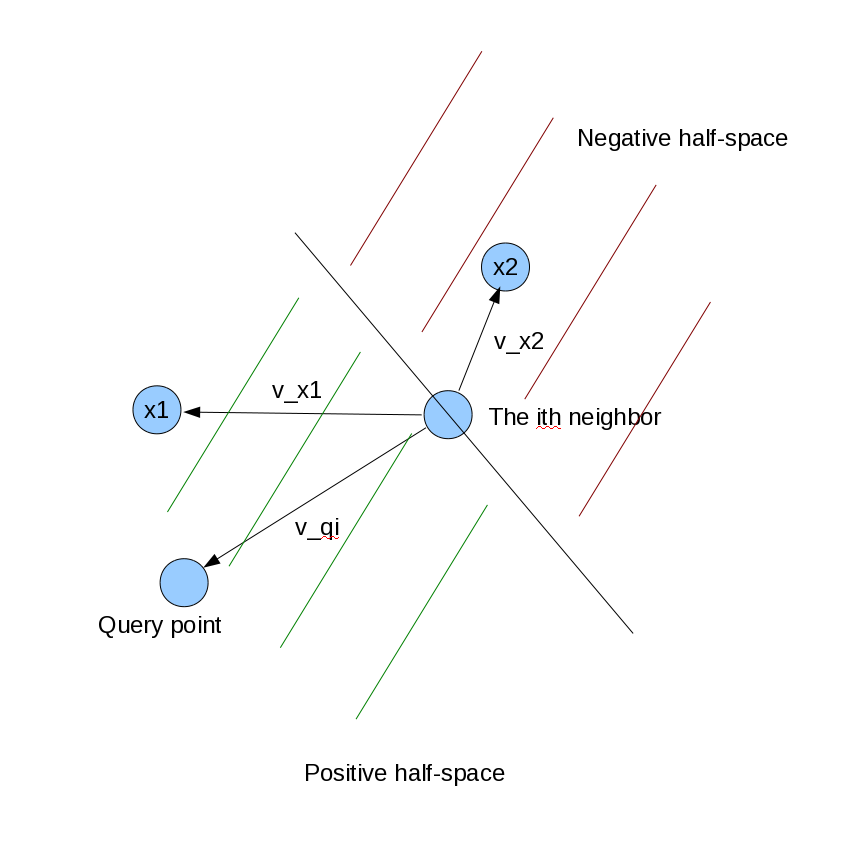
\includegraphics[width=0.4\linewidth]{images/HalfSpace}
  \caption{An example halfspace.}
  \label{fig:HalfSpace}
\end{figure}

Each nearest neighbor point defines a halfspace like this. The BSP neighbors are a subset of the KNearestNeighbors
which are in the intersection of all of the positive halfspaces induced by the kNearestNeighbor points.

Figure \ref{fig:BSPNeighbors} shows an example 2D point set, a query point, and its neighbors. This demo was done in 2D only for clarify of the figure. The method also works in 3D (we have provided Demo3D.cpp to demonstrate this).

\begin{figure}[H]
  \centering
  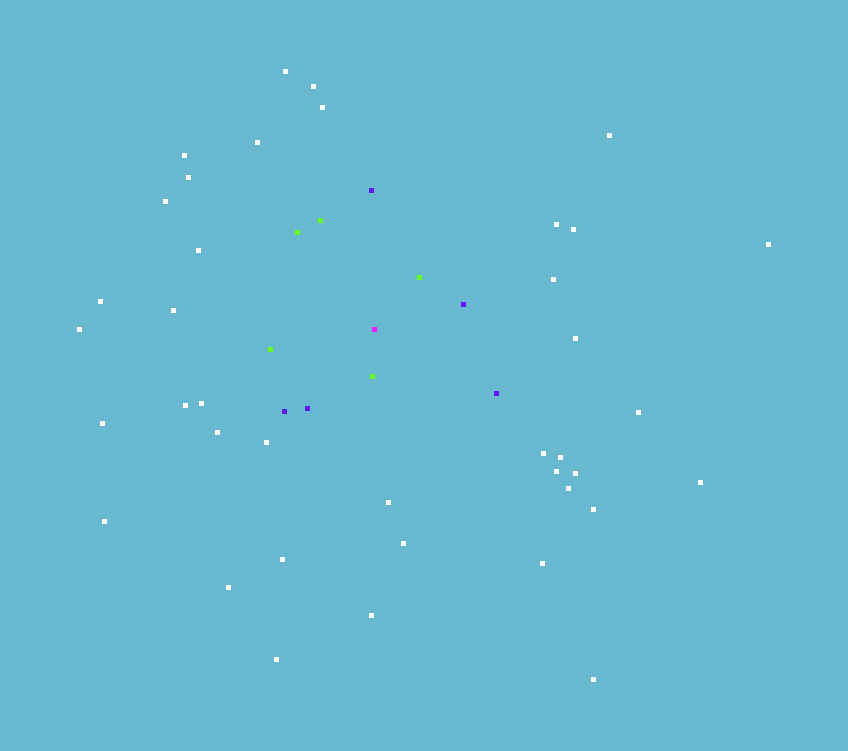
\includegraphics[width=0.4\linewidth]{images/BSPNeighbors}
  \caption{An input point set (white), the query point (pink), BSP Neighbors (green), and KNearestNeighbors that are not included in BSP Neighbors (purple).}
  \label{fig:BSPNeighbors}
\end{figure}

The qualitative effect is that the set of BSP Neighbors has less local duplication, so that each neighbor contributes more information to further computations.

Since this search starts with the K-Nearest neighbors, $K$ must still be specified. However, as long as $K$ is chosen to be large enough, the complete set of BSP neighbors will be found, making this method very insensitive to the parameter as desired.

\subsection{Code Snippet}

\begin{verbatim}
// Find the BSP Neighbors of the point with ID = 0
unsigned int queryPointId = 0;
  
// Create the input point set
vtkSmartPointer<vtkPoints> points = vtkSmartPointer<vtkPoints>::New();
... Fill points2D with points (2D or 3D) ...

// Create an object in which to store the result
vtkSmartPointer<vtkPoints> bspNeighborPoints = vtkSmartPointer<vtkPoints>::New();
    
// Compute the BSP neighbors
BSPNeighbors(reader->GetOutput()->GetPoints(), queryPointId, bspNeighborPoints);
\end{verbatim}


%%%%%%%%%%%%%%%%%%%%
\begin{thebibliography}{9}

	\bibitem{Pauly2003}
	  Pauly, Mark,
	  \emph{Point Primitives for Interactive Modeling and Processing of 3D Geometry}.
	  PhD Thesis, 2003

\end{thebibliography}


\end{document}